% \documentclass[conference]{IEEEtran}
\documentclass[sigconf,screen,balance,natbib=false,timestamp=false,urlbreakonhyphens=true]{acmart}

%\usepackage{cite}  % conflicts with biblatex
\usepackage{amsmath,amssymb,amsfonts}
\usepackage{algorithmic}
\usepackage{graphicx}
\usepackage{textcomp}
\usepackage{xcolor}
\usepackage[utf8]{inputenc}
\usepackage[T1]{fontenc}
\usepackage[hidelinks]{hyperref}
% \usepackage[capitalize,noabbrev]{cleveref} 
\usepackage{microtype}
\usepackage{tabularx}
\usepackage{booktabs}
\usepackage[shortlabels,inline]{enumitem}
\usepackage{xspace}
\usepackage{balance}
\usepackage[colorinlistoftodos,textsize=scriptsize]{todonotes}
\usepackage[type={CC}, modifier={by}, version={4.0}]{doclicense}
\usepackage{listings}
\usepackage{multicol}
\usepackage{biblatex}
\usepackage{subfig}
\usepackage{csvsimple}
\usepackage{multirow}
\usepackage{footmisc}
\usepackage{graphbox}
\usepackage{flafter}
\usepackage{orcidlink}

\addbibresource{IoTcode.bib}


\def\BibTeX{{\rm B\kern-.05em{\sc i\kern-.025em b}\kern-.08em
    T\kern-.1667em\lower.7ex\hbox{E}\kern-.125emX}}
\renewcommand\UrlFont{\color{blue}\rmfamily}
%special custom commands
\newcommand{\specialcell}[2][c]{%
  \begin{tabular}[#1]{@{}c@{}}#2\end{tabular}}

  

%################################################################
\begin{document}
%################################################################
%
\title{Datasets for vulnerabilities detection in IoTs operating systems and applications}

\author{
    Anonymous for review
}

% add IEEE COPYRIGHT here
% \IEEEoverridecommandlockouts
% \IEEEpubid{\makebox[\columnwidth]{978-1-6654-8045-1/22/\$31.00~\copyright2022 IEEE \hfill} 
% \IEEEpubid{\makebox[\columnwidth]{978-1-6654-8045-1/22/\$31.00~\copyright2022 IEEE \hfill} \hspace{\columnsep}\makebox[\columnwidth]{ }}

% CopyRight command
% \IEEEpubidadjcol

\begin{abstract}
TBA
\end{abstract}

% \begin{IEEEkeywords}
  \keywords{
Cybersecurity, Internet of Things, IoT security, Smart Environments, 
Machine Learning, Natural Language Processing;
  }
% \end{IEEEkeywords}

\maketitle

%################################################################
\section{Introduction}
%################################################################

The Internet of Things (IoT) refers to the growing interconnected physical devices, 
components, vehicles and home appliances to the internet~\cite{oracle2023:what}.
These connected devices exchange information to ease our day-to-day lives, business and industries. 
However, these devices continue to pose security issues and vulnerabilities over the years. 



%################################################################
\section{Related Work}
%################################################################

Al‑Boghdady et al.~\cite{al-boghdady2022:idetect} have created a tool called iDetect for detecting 
vulnerabilities in the C/C++ source code of IoT operating systems (OSs). 
The labeling of the dataset was done using static code analyzing tools (SATs);
Cppcheck version 2.1~\cite{cppcheck2.12021:tool}, 
Flawfinder version 2.0.11~\cite{dwheeler2021:flawfinder}, 
and Rough Auditing Tool for Security (RATS)~\cite{rats2021:rough}.



%################################################################
\section{The proposed framework:}
%################################################################

\begin{figure}[h!]
  \centering
  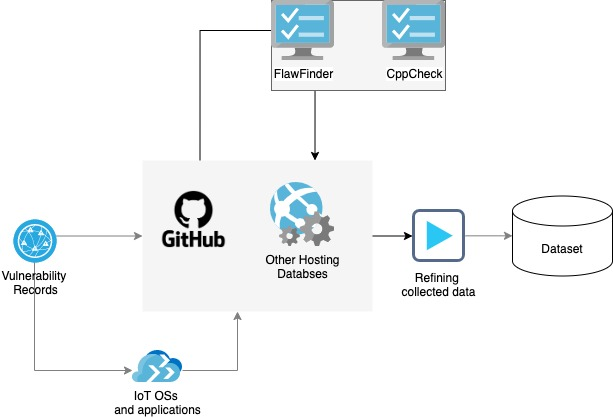
\includegraphics[width=8cm]{../figure/framework.jpg}
  \vspace*{-1.5ex}
  \caption{The proposed framework for vulnerability data collection}
  \label{fig:lcurve-iot}
\end{figure}


%################################################################
\section{Dataset Analysis:}
%################################################################

% % importing CSV file: ../result/top-databases.csv
\begin{table*}[!t]
  \centering
  \csvreader[
    tabular=|m{4cm}|m{1cm}|,
    /csv/separator=semicolon,
    table head=\hline \bfseries{urls} & \bfseries{count}  \\\hline,
    late after line=\\\hline, 
  ]
  {../result/top-databases.csv}{}
  {\csvlinetotablerow}
  \caption{Summary of the top databases hosting vulnerability records of IoT OSs and applications}
  \label{tab:software}
  \end{table*}


  \begin{figure}[h!]
    \centering
    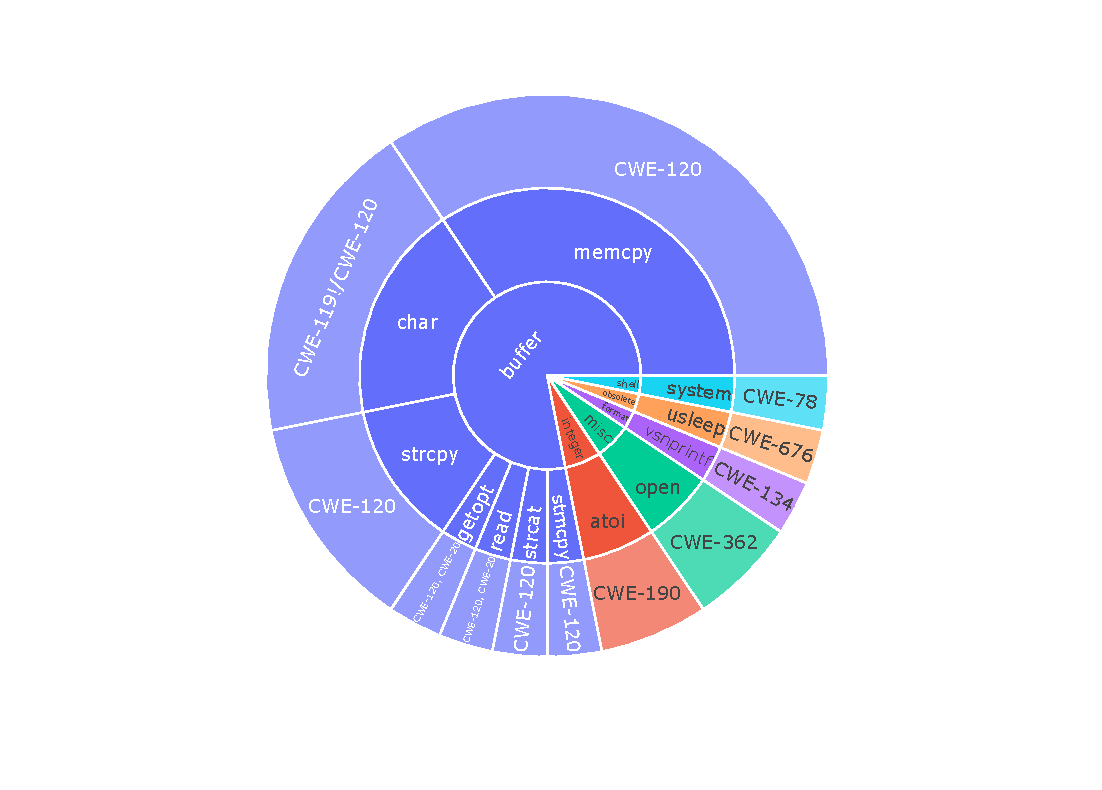
\includegraphics[width=10cm]{../figure/vul_sunburst.pdf}
    \vspace*{-1.5ex}
    \caption{The sunburst chart showing the frequency of vulnerability categories, names and CWEs}
    \label{fig:lcurve-iot}
  \end{figure}


%################################################################
\section{Conclusion and Future Work}
%################################################################
\label{conclusion}



\printbibliography
\end{document}
